\begin{problem}{Sort}{Inn}{Út}{~}{~}

	\begin{wrapfigure}{r}{0.25\textwidth}
		\vspace{-25pt}
		\begin{center}
			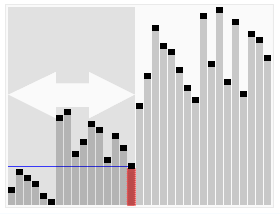
\includegraphics[scale=0.40]{../Sort/sorting.png}
		\end{center}
		\vspace{-30pt}
	\end{wrapfigure}

	Margar forritunarkeppnir hafa dæmi þar sem keppendur eiga að raða lista af heiltölum. Þetta dæmi er aðeins öðruvísi, en hérna eigið þið að dæma lausnir á röðunarverkefninu.

	Þið fáið gefna tvo lista af heiltölum. Fyrri listinn er ekki í neinni sérstakri röð, og er það listinn sem keppendur eiga að raða. Seinni listinn er hugsanlega raðaða útgáfan af fyrri listanum, en hann er svar frá einhverjum keppanda við fyrri listanum.

	Skrifið forrit sem ákvarðar hvort seinni listinn sé raðaða útgáfan af fyrri listanum eða ekki.

	\Input

		Á fyrstu línu er heiltalan $1 \leq T \leq 1000$, sem táknar fjölda prófunartilvika sem fylgja. Hvert prófunartilvik samanstendur af tveimur línum, sem hvor um sig hefur eina eða fleiri heiltölur aðskildar með bili.

	\Output

		Fyrir hvert prófunartilvik á að skrifa út eina línu sem inniheldur "`\texttt{Accepted}"' ef seinni listinn er raðaða útgáfan af fyrri listanum, en "`\texttt{Wrong Answer}"' annars.

	\Examples

		\begin{example}
			\exmp{
4
2 3 1 4
1 2 3 4
10 -8 4 7 7 8 9
-8 4 7 7 9 8 10
10 11 12
10 11 12
1 2 3 4
5 6 7 8
			}{
Accepted
Wrong Answer
Accepted
Wrong Answer
}%
		\end{example}

	\Explanation

		\begin{enumerate}
			\item Listinn \texttt{1 2 3 4} er augljóslega raðaða útgáfan af listanum \texttt{2 3 1 4}, og þess vegna er svarið \texttt{Accepted}
			\item Svarið væri \texttt{Accepted} ef skipt væri á 8 og 9
			\item Listinn var raðaður, og er rétta svarið því listinn sjálfur. Þetta gefur því \texttt{Accepted}
			\item Seinni listinn er ekki raðaða útgáfan af fyrri listanum, en hann inniheldur ekki einu sinni sömu heiltölur
		\end{enumerate}

\end{problem}